\chapter{Method}
\section{Deep HAR}

In the previous chapter, approaches for estimating pose from still images and predicting actions from video were presented.
Although some approaches for HAR incorporate pose information as features in their decision process, estimating pose and predicting actions were not used in conjunction during the training process.
For example, \cite{choutas_potion:_2018} \sref{sec:potion} estimated pose using a dedicated model, before using the information to train their model. 

This chapter presents the approach by \cite{luvizon_2d/3d_2018}, who argue that estimating pose and predicting action in a single model may help in the learning process, since the pose estimator can incorporate action prediction information and vice versa.
In Section \ref{sec:softargmax}, the authors present a novel way to infer joint coordinates from heatmap, which allows the model to be fully differentiable and thus able to be trained in an end-to-end approach.
Next, the model architecture the authors used is presented in Section \ref{sec:deephar_architecture}.
For training the model, the authors use an approach called \textit{intermediate supervision}, which is presented in Section \ref{sec:luvizon_intermediate_supervision}.
Lastly, this thesis presents limitations of the authors work in Section \ref{sec:deephar_limitations}, in addition to proposed experiments to overcome some of those limitations.

\subsection{Approach}
\label{sec:deephar_approach}

In \cite{luvizon_2d/3d_2018}, the authors propose a network, which estimates pose and then uses the estimation, in combination with low level image features, to predict the action performed by a subject in a video clip.
The network is completely differentiable, which allows the authors to pretrain certain parts, like the post estimator, and then fine-tune the network in an end-to-end fashion.
They claim that such an approach is novel and has never been attempted because state-of-the-art pose estimators at that time where not fully differentiable.
This is because they output a heatmap, like the Stacked Hourglass network \cite{newell_stacked_2016} \sref{sec:stacked_hourglass}, for each joint position.
Such a heatmap requires the use of the argmax function in a postprocessing step to compute the $x$ and $y$ values of the highest peak.
Thus, the authors propose the \textit{Soft-argmax} function as an differentiable alternative to the regular argmax function \sref{sec:softargmax}.

In addition, the authors propose methods to use both $3D$ and $2D$ pose datasets while training their network.
However, these are not discussed here since this thesis focuses on $2D$ pose information. 

\subsection{Soft-argmax}
\label{sec:softargmax}
The authors propose an approach for computing the $x$ and $y$ coordinates from a joint heatmap using a method called \textit{Soft-argmax} \cite{luvizon_human_2017}.
After computing the Softmax $\Phi(h)$ of a joint heatmap $h$, $x$ and $y$ coordinates of the maximum need to be regressed to be able to fine-tune the network in an end-to-end fashion since the regular argmax function is not differentiable \cite{luvizon_2d/3d_2018}.
This is achieved by computing the expectation in $x$ and $y$ direction on the probability map produced by the Softmax function.
In the implementation, the authors first define a fixed weight matrix for a convolutional layer in the following way:

\begin{figure}[htb!]
    \centering
    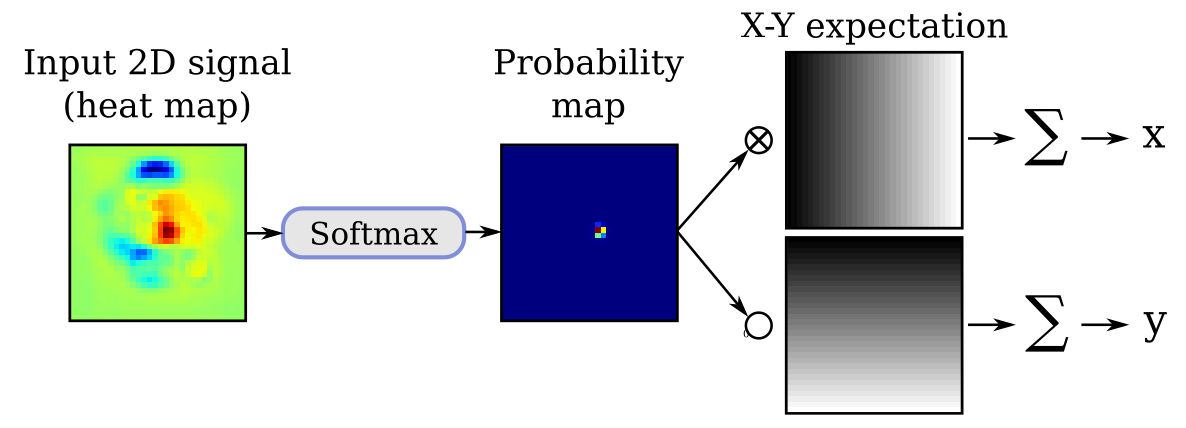
\includegraphics[width=0.6\textwidth]{softargmax_pipeline.png}
    \caption{The approach presented by the authors to regress $x$ and $y$ coordinates from heatmaps. First, they apply a Softmax. Then, they compute the expectation in both $x$ and $y$ direction using a \textit{2D ramp function}. Summation of the result then leads to the regressed coordinates. Image taken from \cite{luvizon_2d/3d_2018}. }
    \label{fig:softargmax_pipeline}
\end{figure}

\begin{equation}
    \bm{W}_{i,j,x} = \frac{i}{W}, ~ \bm{W}_{i,j,y} = \frac{j}{H},
\end{equation}

where $H, W$ refer to the width and height of the heatmap and $i,j$ are the coordinates for each element in the heatmap.
This leads to ramp functions for the horizontal and vertical dimensions, which are visualized in \fref{fig:softargmax_pipeline}.
By convolving a part heatmap with both $\bm{W}_x$ and $\bm{W}_y$ the expectations are computed, leading to the regressed coordinate $(\psi_x(h), \psi_y(h)) = ((x_{exp}, y_{exp})$ with $x_{exp}, y_{exp} \in [0,1]$ (see \eref{eq:softargmax_conv}).
The regressed coordinates need to be multiplied with the width and height in order to obtain integer coordinates.

\begin{equation}
    \label{eq:softargmax_conv}
    \psi_d(h) = \sum_{i=1}^W \sum_{j=1}^H \bm{W}_{i,j,d} \Phi(h_{i,j})
\end{equation}

The authors further prove that the Soft-argmax function is differentiable by providing the derivative of $\psi_d(h)$:

\begin{equation}
    \frac{\partial \psi_d(h_{i,j})}{\partial h_{i,j}} = \bm{W}_{i,j,d} \frac{ exp(h_{i,j}) (\sum_{k=1}^W \sum_{l=1}^H exp(h_{k,l} - exp(h_{i,j}) ) } { ( \sum_{k=1}^W \sum_{l=1}^H exp(h_{k,l}) )^2 }
\end{equation}

Further, the authors argue that such a method for regressing $x$ and $y$ coordinates is more accurate and requires fewer training weights than directly regressing them using, for example, a fully-connected layer \cite{luvizon_human_2017}.
As proof, they compare their methods to other state-of-the-art methods which directly regress the coordinates, and observe that their approach consistently outperforms these approaches on the MPII benchmark.
Specifically, when comparing to the previously best approach for regressing pose by \cite{sun_compositional_2017}, the authors observe an overall increase in PCKh accuracy of $5.2$ percentage points from $86.4$ to $91.2$ percent.

\subsection{Architecture}
\label{sec:deephar_architecture}

The architecture used by the authors can be divided into several blocks.
First, a feature extraction block, referred to as \textit{Stem}, is used to extract visual features from each frame of the input video separately.
Afterwards, these features are used to predict the joint heatmaps in the pose estimation block.
The heatmaps are then used to compute the $x$ and $y$ coordinates of each joint position using the Soft-argmax function.
Then, the network splits into two action recognition pipelines.
In the first pipeline, further referred to as \textit{Pose Model}, the pose coordinates for all frames in the video clip are aggregated into a matrix and the action is predicted on this matrix.
In the second pipeline, further referred to as \textit{Visual Model}, the image features from the \textit{Stem} block are aggregated in a similar fashion to the \textit{Pose Model} into a matrix, which is also used to predict the performed action.
Finally, both intermediate action predictions are combined to form the final prediction.
Throughout the entire network, the authors use the ReLU activation function if not otherwise stated.
See \fref{fig:luvizon_overview} for a visualization of the network and its separate components.

\begin{figure}[htb!]
    \centering
    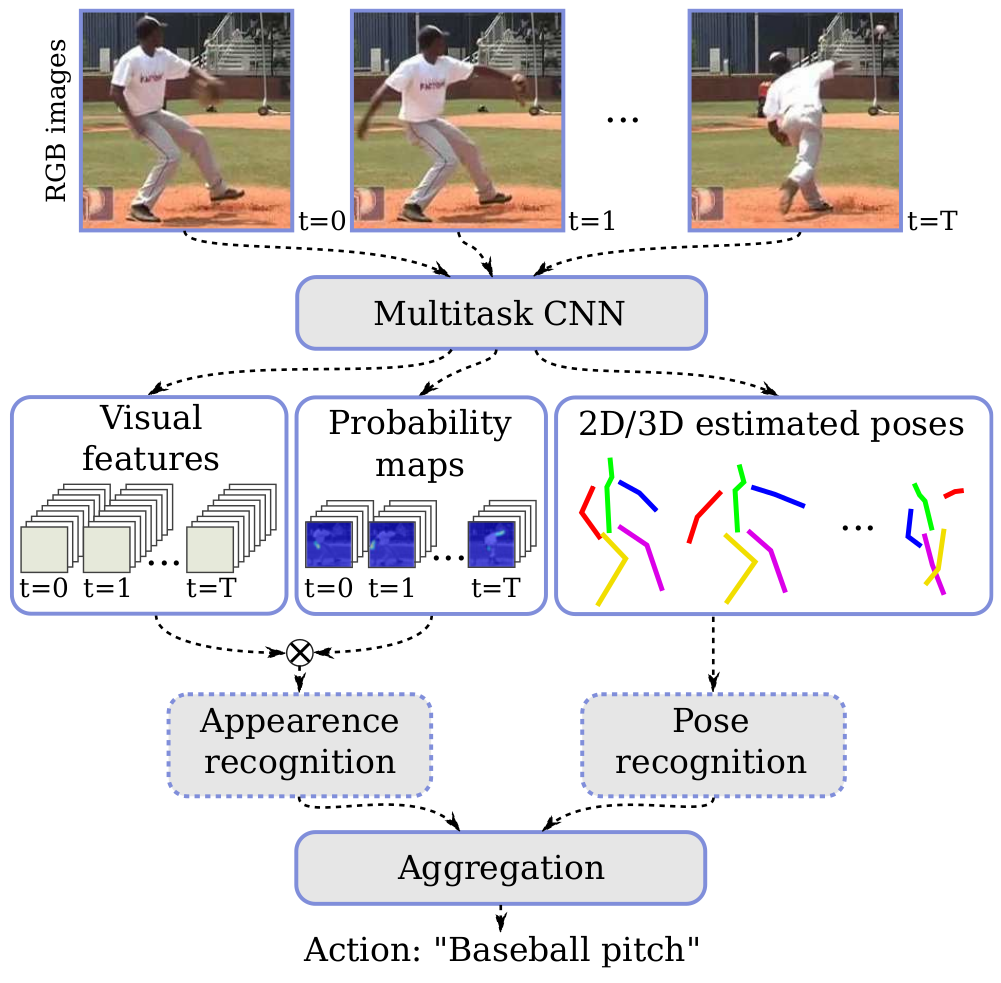
\includegraphics[width=0.6\textwidth]{endtoend-concept.png}
    \caption{High level visualization of the network used by \cite{luvizon_2d/3d_2018}. The images features and poses are computed frame-by-frame. The output is then passed to the appearance and pose recognition subnetworks, where they are jointly processed to predict the action of the video clip. Image taken from \cite{luvizon_2d/3d_2018}.}
    \label{fig:luvizon_overview}
\end{figure}

\subsubsection{Feature extraction (Stem)}
The authors base their feature extraction network off of the \textit{Inception v4} network proposed by \cite{szegedy_inception-v4_2017}.
One addition the authors made was to use a final \textit{depthwise separable convolutional layer} at the end of the network.

A \textit{depthwise separable convolution} \cite{sifre_rigid-motion_2014} \cite{chollet_xception:_2017} is used to reduce the number of parameters and matrix multiplications needed for convolutional layers with many channels.
Consider an input matrix (like an RGB image) to a convolutional layer of size $n \times n \times p$, where $p$ indicates the number of channels.
Without loss of generality, a square input as well as a square kernel size is assumed.
If a regular convolutional layer is used, and the desired number of output channels is given by $m$ with $m \gg p$, then one approach is to use $m$ kernels in the convolutional layer of size $a \times a \times p$.
This results in $a^2 * p * m$ parameters of the convolutional layer which need to be learned.
In a depthwise separable convolutional layer, two convolutional layers are used after one another, referred to as the \textit{depthwise convolutional layer} and \textit{pointwise convolutional layer}.
The \textit{depthwise convolutional layer} uses $p$ filters of size $a \times a \times 1$ to process the input matrix one channel at a time.
Afterwards, the \textit{pointwise convolutional layer} uses $m$ filters of size $1 \times 1 \times p$.
This results in $$p * m + p * a^2 \Leftrightarrow p * (m + a^2)$$ learnable parameters for both convolutional layers.
It is then easy to see that $$p * (m + a^2) \ll p * m * a^2.$$
Additionally, the number of matrix multiplications needed to compute the convolution is reduced significantly as well.
Let $b$ be the number of multiplications performed on either $x$ or $y$ dimension on an matrix of size $n \times n$ using a kernel of size $a \times a$.
The number of matrix multiplications necessary in a regular convolutional layer is equal to $a^2 * b^2 * p * m$.
In a depthwise separable convolutional layer, the number of multiplications reduces to $a^2 * b^2 * p $ for the depthwise and $b^2 * m * p$ for the pointwise convolutional layer.
This results in $$a^2 * b^2 * p + b^2 * m * p \Leftrightarrow b^2 * (a^2 * p + p * m) $$ overall multiplications.
To show that the number of multiplications needed is lower, it needs to be shown that $a^2 * p + p * m < a^2 * p * m$ (see \eref{eq:convolution_proof}).
The assumption holds since $a \ll m$.

\begin{equation}
    \label{eq:convolution_proof}
    \begin{split}
        &a^2 * p + p * m < a^2 * p * m \\
        &\Leftrightarrow p * (a^2 + m) < p * a^2 * m \\
        &\Leftrightarrow a^2 + m < a^2 * m  
    \end{split}
\end{equation}

\begin{figure}[htb!]
    \centering
    \subfloat[\textit{Stem} network. ]{
        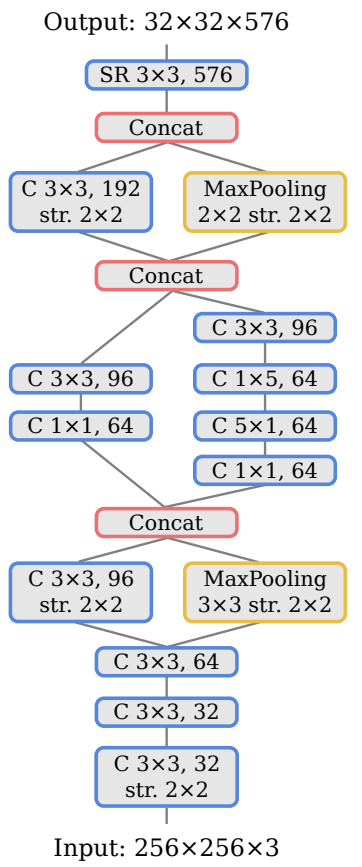
\includegraphics[width=0.3\textwidth]{luvizon_stem.png}
        \label{fig:luvizon_stem}
    }
    \hfill
    \subfloat[\textit{Prediction block} network]{
        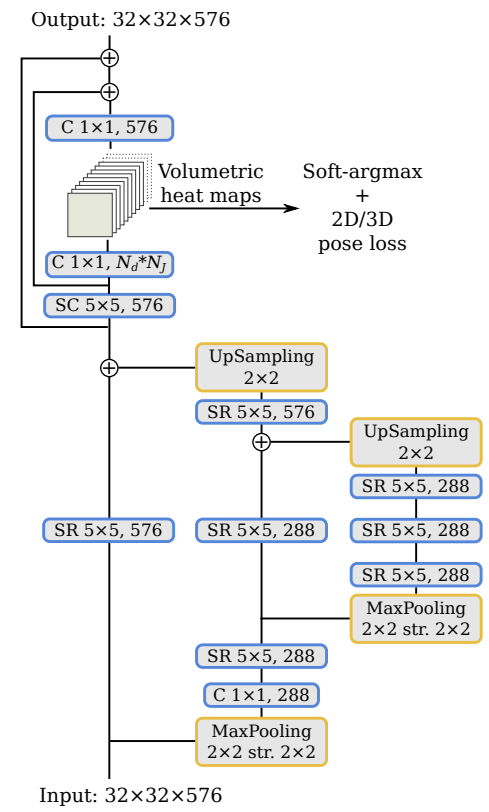
\includegraphics[width=0.5\textwidth]{luvizon_predictionblock.png}
        \label{fig:luvizon_predictionblock}
    }
    \caption{\textbf{Left:} The feature extraction network used in \cite{luvizon_2d/3d_2018}, also referred to as \textit{Stem}. Each RGB frame of the video is resized to $256 \times 256 \times 3$. \textit{SR} refers to a \textit{depthwise separable convolution}. \textit{C} refers to a regular convolutional layer. The extracted features are of size $32 \times 32 \times 576$. 
    \textbf{Right:} One \textit{prediction block} used in the pose estimation network in \cite{luvizon_2d/3d_2018}. Notice that the input and output dimensionality are identical, which allows the authors to connect multiple blocks together. \textit{C} and \textit{SC} refer to regular convolutional layers and depthwise separable convolutional layers, respectively. \textit{SR} refers to a \textit{Separable residual block}. The estimated pose of each prediction block can then also be used for intermediate supervision \sref{sec:luvizon_intermediate_supervision}. Images taken from \cite{luvizon_2d/3d_2018} supplementary material.}
\end{figure}

\subsubsection{Pose estimation}
\label{sec:luvizon_poseestimator}
For the pose estimation network, the authors build upon the work by \cite{newell_stacked_2016} (see \sref{sec:stacked_hourglass}).
Their pose estimator is constructed from multiple \textit{prediction blocks}, which are visualized in \fref{fig:luvizon_predictionblock}.
Similar to the stacked hourglass architecture, the prediction block computes features on different scales of the input by utilizing \textit{Max-pooling} and \textit{Upsampling} layers.
In particular, the authors use \textit{separable residual blocks} in place of regular convolutions to extract these scale-dependant features.

A \textit{separable residual block} is defined by the authors in their previous work \cite{luvizon_human_2017} as a depthwise separable convolutional layer, whose input is added to the output using a residual connection (see \sref{sec:residual_blocks}).
For the case where the number of output channels $p_{out}$ is different to the number of input channels $p_{in}$, the authors add a convolutional layer with $p_{out}$ kernels of size $1 \times 1 \times p_{in}$ to ensure that the addition of the input with the output of the depthwise separable convolutional layer is possible.
The authors do not, however, motivate their decision for using such separable residual blocks.

After the extraction of features on different scales, the features are passed to a convolutional layer with $N_j + N_j * N_c$ filters of size $1 \times 1 \times 576$, which leads to the output of $N_j + N_j * N_c$ heatmaps of size $32 \times 32$.
$N_j$ refers to the number of desired heatmaps, i.e., the number of joints that need to be detected.
$N_c$ is defined by the authors as the number of additional heatmaps per joint heatmap, called \textit{context heatmaps}.
This means that $N_c + 1$ heatmaps are computed per joint.
The Soft-argmax then computes the predicted joint locations on all heatmaps and aggregates the results for each joint using \eref{eq:context_sum}.
There, $\alpha \in [0,1]$ determines how much influence the context heatmaps $(\bm{h_{1,n}}, \dots, \bm{h_{N_c, n}}$ should have on the prediction of the joint $n \in [1, N_j]$.
$SA$ refers to the Soft-argmax function, computing joint position estimates from heatmaps.
Additionally, $\bm{p}_n$ refers to the predicted visibility of joint $n$, which the authors estimate by using Max-pooling on heatmap $\bm{h}_n$, followed by a sigmoid activation function.
In \cite{luvizon_human_2017}, the authors present this approach and argue that, for the final joint location prediction, this approach leads to more accurate results, without specific evaluation of accuracy with and without context heatmaps.

\begin{equation}
    \label{eq:context_sum}
    y_n = \alpha \cdot SA(\bm{h}_n) + (1 - \alpha) \frac{\sum_{i=1}^{N_c} \bm{p}_{i,n} \cdot SA(\bm{h}_{i,n}) }{\sum_{i=1}^{N_c} \bm{p}_{i,n} }.
\end{equation}

Similar to the stacked hourglass approach by \cite{newell_stacked_2016}, the prediction block is designed in a way that the input and output dimensions are identical, which allows the authors to connect multiple prediction blocks together.
When training the pose estimator for evaluating its accuracy, the authors choose to use $8$ prediction blocks, whereas a smaller pose estimator of $4$ blocks is used when incorporating it into the human activity recognition pipeline.
The authors do not motivate their choices or evaluate the accuracy of different number of prediction blocks, which is why we chose to evaluate the accuracy experimentally in \sref{sec:exp-replication}.

\subsubsection{Pose Model}
\label{sec:pose_based_action_recognition}
\begin{figure}[htb!]
    \centering
    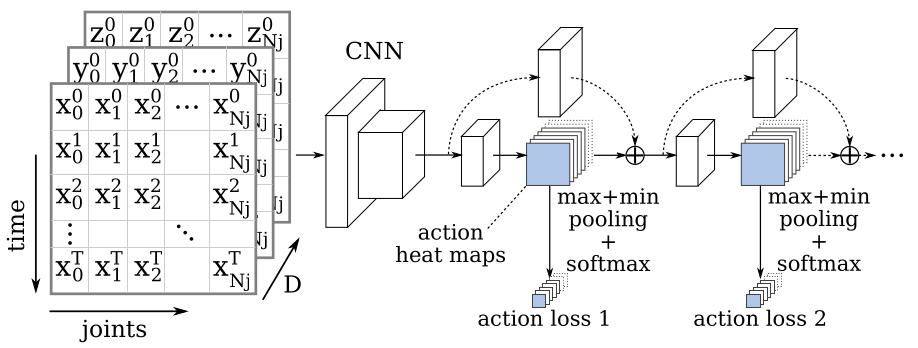
\includegraphics[width=0.60\textwidth]{luvizon_poseaction.png}
    \caption{The approach presented by \cite{luvizon_2d/3d_2018} to aggregate the estimated pose for each frame and use it to estimate the performed action. The chosen pose representation is also referred to as a \textit{pose cube}, since represents a three dimensional matrix. Notice that the pipeline produces intermediate action recognition results, which can be used for intermediate supervision \sref{sec:luvizon_intermediate_supervision}. Image taken from \cite{luvizon_2d/3d_2018}.}
    \label{fig:luvizon_poseaction}
\end{figure}

After computing image features in the \textit{Stem} network and feeding them into the pose estimator, the authors decide to split their network into two parts for estimating the performed action.
The first path, further referred to as \textit{Pose Model}, aggregates the predicted $x$ and $y$ coordinates for each frame of the input video into a three-dimensional matrix representation of size $a \times b \times z$, also referred to as the \textit{pose cube}.
$b$ refers to the number of frames of the input clip, while $a$ determines the number of joints to detect.
To ensure that the pose matrix has identical dimensionality, regardless of the original input video length, the authors decide to subdivide the video into chunks of $16$ frames, resulting in $b=16$.
The last dimension stores the $x$ and $y$ coordinates, respectively, resulting in $z=2$ and a total dimensionality of $16 \times 16 \times 2$, since all datasets are processed in a way to ensure that there are always $16$ joints (see \sref{sec:exp-datasets} for a more detailed explanation).
An alternative representation to the pose cube is evaluated in \sref{sec:different_pose_representation_experiment}.
Afterwards, the pose cube is processed by a fully-convolutional neural network, which can be seen in \fref{fig:luvizon_actionrecognitionblock}, before being fed into a so called \textit{action prediction block}.
The authors decide to use a function called \textit{MaxPlusMin pooling} instead of regular \textit{Max-pooling}.
This function is implemented by the authors using a \textit{Max-pooling} operation with kernel size $(4,4)$ in the following way:

\begin{equation}
    MaxMinPooling(x) = MaxPool(x) - MaxPool(-x).
\end{equation}
However, the authors do not explain the benefit of such a pooling operation over a regular \textit{Max-pooling} layer.

\begin{figure}[htb!]
    \centering
    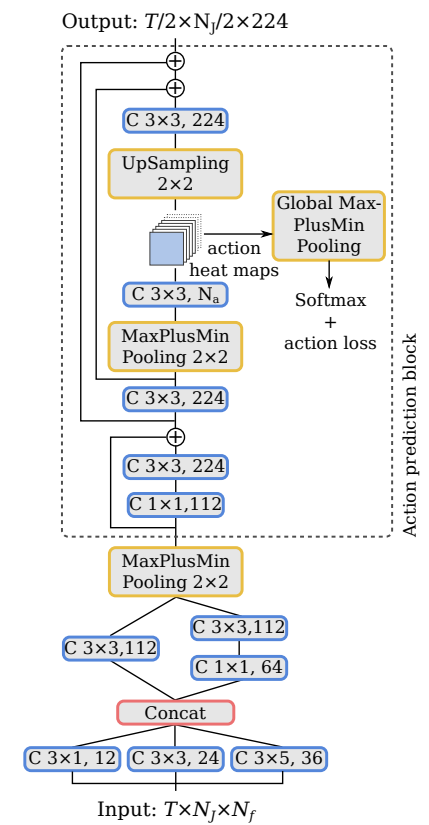
\includegraphics[width=0.45\textwidth]{luvizon_actionrecognitionblock.png}
    \caption{The fully-convolutional network used to process the \textit{pose cube}, followed by a single \textit{action prediction block}. $T$ refers to the number of frames, $N_j$ is defined as the number of joints and $N_f$ represents the third dimension, i.e., $2$ in the case of the pose cube. In the action prediction block, the number of actions to detect can be set using $N_a$. Image taken from \cite{luvizon_2d/3d_2018} supplementary material.}
    \label{fig:luvizon_actionrecognitionblock}
\end{figure}

The purpose of the fully-convolutional block is to extract features from the pose matrix.
Afterwards, a processing block called \textit{action prediction block} can be used to classify the action performed, based on the features computed from either pose or appearance cube. 

The \textit{action prediction block} is similar to the \textit{prediction block} used in the pose estimator, and again follows the ideas of stacking, since input and output dimensions of the action prediction block are identical.
As an intermediate representation, \textit{action heatmaps} are created, which are in turn used to predict the action performed in the video clip using the Softmax activation function.
Notice that the output of the action prediction block is not the predicted action itself, but rather features of the same dimensionality as the input to the block.
The predicted actions are only used for computing the loss during training and are not passed further through the network.

\subsubsection{Visual Model}
\begin{figure}[htb!]
    \centering
    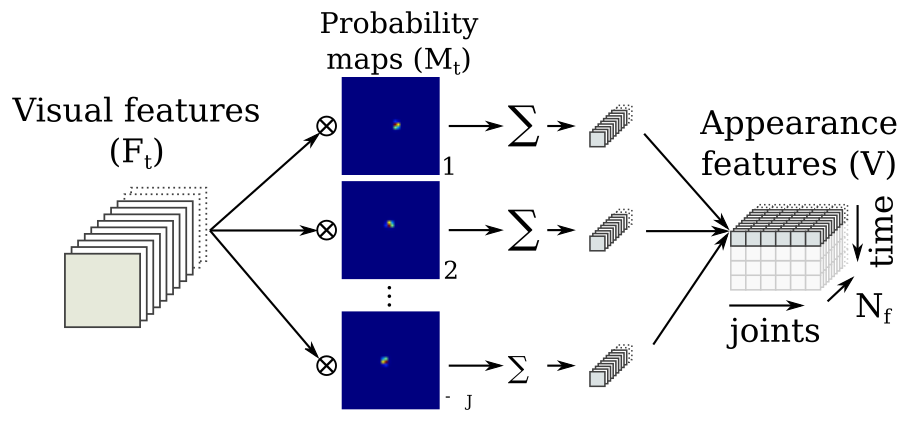
\includegraphics[width=0.6\textwidth]{luvizon_appearanceaction.png}
    \caption{The approach proposed in \cite{luvizon_2d/3d_2018} to aggregate image features for multiple frames into a \textit{appearance cube}. This cube can then be used for further processing, similar to the \textit{pose cube}. Image taken from \cite{luvizon_2d/3d_2018}.}
    \label{fig:luvizon_appearanceaction}
\end{figure}

\begin{figure}[htb!]
    \centering
    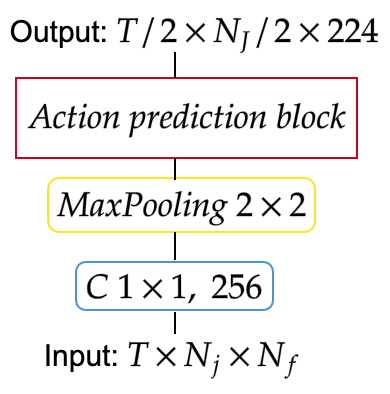
\includegraphics[width=0.3\textwidth]{luvizon_appearancebasedaction.png}
    \caption{The \textit{Visual Model}, according to the code provided as supplementary material to \cite{luvizon_2d/3d_2018}. The architecture differs to the one presented in the paper, where the authors claim that both \textit{Visual Model} and \textit{Pose Model} have identical architectures.}
    \label{fig:luvizon_appearancbasedeaction}
\end{figure}

The authors also want to incorporate low level image features from the \textit{Stem} block into their action recognition approach, in addition to estimated pose information.
Thus, they aggregate the computed visual features for each frame in a similar way to the pose cube.
This is referred to as the \textit{appearance cube}.
The computed features $f_d$ for a frame $d$ have the dimensionality $32 \times 32 \times 576$.
The authors then multiply $f_d$ with each computed joint heatmap, after the heatmaps were further processed by applying the Softmax activation function.
Notice that they do not multiply the features with the context heatmaps, but only with the $N_j$ joint heatmaps.
Afterwards, the resulting features are summed over the first two dimensions, resulting in a new feature of size $1 \times 1 \times 576$.
Then, these new features are aggregated into the appearance cube, resulting in a cube of dimensionality $16 \times 16 \times 576$.
See \fref{fig:luvizon_appearanceaction} for a visualization of this process.
The authors then use a different feature extraction step as in the \textit{Pose Model}.
Noticeably, the feature extraction consists of a single convolutional layer, followed by a batch normalization and a \textit{Max-pooling} layer.
In \cite{luvizon_2d/3d_2018}, the authors claim that they use a similar architecture to the \textit{Pose Model}.
However, when examining the code published as supplementary material, we found that they actually use the shallow model mentioned before.
A visualization of the shallow feature extractor can be seen in \fref{fig:luvizon_appearancbasedeaction}.
The action prediction block is then again identical to the one presented in the \textit{Pose Model} (see \fref{fig:luvizon_actionrecognitionblock}).

For combining both the predictions based on the pose cube and appearance cube, the authors take the output of the last action prediction block in both networks, add the activations and apply a final \textit{Max-Pooling} and Softmax activation to form the final result. 

\subsection{Intermediate supervision}
\label{sec:luvizon_intermediate_supervision}
One aspect of the training process the authors use is called \textit{intermediate supervision}.
Instead of only using the final output of the network to compute the error and start the backpropagation algorithm, multiple intermediate results are created, each of which can then be used to compute the error and start backpropagation.
After each prediction block in the pose estimator, a intermediate prediction is performed by applying Soft-argmax to the joint heatmaps created by that prediction block.
Similarly, in each action prediction block, intermediate results are created by performing pooling and Softmax to the action heatmaps, which can be seen in \fref{fig:luvizon_poseaction}.
The authors claim that this approach increases the accuracy of the overall network, since the network needs to be able to predict the action as early and as accurately as possible.
However, they do not provide evidence to proof their claim.  

\subsection{Limitations}
\label{sec:deephar_limitations}
There are four limitations to the approach proposed by the authors and their evaluation of the method.
First, they imply by the choice of their paper's title that their approach constitutes end-to-end learning.
This would imply that the network weights are not pretrained in any way.
However, as discussed earlier, the pose estimator is pretrained.
While this approach leads to competitive results, it is misleading to call it end-to-end training.
Later in their paper, the authors refer to their approach as fine-tuning on a pretrained model, which is more a more accurate description of the process. 

Second, the authors evaluate their model for $2D$ action recognition solely on the Penn Action dataset.
While they do not focus exclusively on $2D$ action recognition in their paper, a comparison to state-of-the-art results on other complex datasets such as JHMDB would be desirable.
This is especially true considering that Penn Action focuses on $15$ different actions, which are predominantly from the sports domain, while JHMDB contains $21$ classes, including every day activity such as \textit{brushing hair} and \textit{climb stairs}.
We thus argue that evaluation on the JHMDB dataset will lead to valuable insight into the effectiveness of the authors approach outside of the domain of sports action recognition. 

Third, an evaluation of choices the authors made regarding certain hyperparameters is not given in the original work.
For example, the authors decided to utilize context heatmaps (as discussed in \sref{sec:luvizon_poseestimator}) as well as setting the number of prediction blocks of their pose estimator to $8$.
They do not provide explanations or evaluations as to why these decisions were made and thus further analysis will give a better insight into the differences these choices make considering the overall quality of the model.

Fourth, the pose estimator used by the authors processes the input videos frame by frame.
This means that temporal information, which could aid in pose estimation, is not utilized for training.
As an example, \cite{girdhar_detect-and-track:_2018} adopt a frame by frame approach to video data by incorporating $3D$ convolutional layer to capture temporal information.
They show an increase in accuracy when comparing predicting the pose for each frame individually, suggesting that capturing the temporal dimension can aid in learning pose in videos.

\section{Proposed experiments}
Apart from recreating some key findings of the authors and evaluating certain decisions by the authors as explained before, we propose two extensions to the network architecture and learning process.

First, we propose to combine the losses of the pose estimator with the losses of the overall action recognition pipeline in a similar manner to the intermediate supervision approach.
A combination of the loss function allows for the network to be trained in an end-to-end fashion, as opposed to fine-tuning the network after pretraining certain components.
This will give an insight not only into the feasibility of the end-to-end training approach but also on the results regarding the pose estimator.
\cite{iqbal_pose_2016} argue that pose estimation accuracy increases when given an action prior.
Also, in the approaches discussed earlier \sref{sec:har_using_pose}, using pose information for action recognition significantly increases the overall accuracy.
Thus, we propose that, by using an end-to-end learning approach, both pose estimation and action recognition networks could benefit from each other when learned jointly.

Second, recent work utilize information gathered by \textit{Inertial Measurement Units (IMUs)} for action recognition in a warehouse setting \cite{reining_towards_2018}.
IMUs are physical devices attached to a subjects body, containing accelerometers, gyroscopes and magnetometers.
These sensors measure time-series data which are then used for action recognition.
We propose to change the encoding of the estimated pose into a similar, time-series representation, so that it can be used with IMU data in future work.
In addition, since the authors did not evaluate different methods for encoding video pose information, this will lead to more insight into how such an encoding effects the overall performance of the network.
